% Experiments for the current decoder and explicitly separated historical arms.
\section{Experiments}
\label{sec:experiments}
We report two distinct numerical collections. A new 60-graph audit evaluates
the current full-Bernoulli Algorithm~1: global-mean growing followed by
at most $\lceil\log n\rceil$ rounds of deterministic parameter replacement
and a mandatory final M-step. The earlier 240-graph collection evaluates
historical sparse-score procedures and is preserved under its original
protocol. The two collections use different scores, clipping rules, and
fitting budgets; their results are reported separately. We also give an
exactly certified population example explaining why a guarantee for growing
alone cannot permit arbitrary finite intermediate EM budgets.

\subsection{Current full-Bernoulli decoder: design and comparisons}
The new design contains $n=320$ vertices and
$K\in\{2,3,4,5,6\}$, three matrix families, two density settings, and two
independent graph seeds per cell, giving $5\times3\times2\times2=60$ graphs.
The families are a balanced assortative model, an unequal-size
disassortative model, and an unequal-size weak general model. Their block
matrices are entrywise positive, symmetric, and full rank. The second family
has negative signal eigenvalues; the third includes directions with weak
finite-sample separation. The exact matrices, block sizes, and seeds are
fixed in the saved protocol.

Each probability matrix is scaled so that the average expected degree,
computed using the actual integer block sizes and excluding self-loops,
equals either $3\log n$ or $0.18(n-1)$. Expected degrees may differ between
blocks. Both density settings use the same decoder and score; no adjacency
regularization or edge-based refinement is applied.

Every method receives the same $K$ raw adjacency eigenpairs with largest
absolute eigenvalues. The full-score and sparse-score controls use exactly
the same clipped reconstruction $q$. For this audit the clipping endpoints
are $\varepsilon$ and $1-\varepsilon$, where
\[
 \varepsilon=10^{-4}\frac{\max\{1,\max_a|\Lambda_{aa}|\}}n.
\]
The reconstructed diagonal is retained. Thus the score-family comparison
changes the working criterion while keeping the spectral information and
clipping identical. It is not a comparison of graph likelihoods computed
from different observations.

For each score family, the growing fit takes at most 100 EM updates at
each stage, with unchanged labels and soft-loss change at most $10^{-9}n$
required for early stopping. Replacement tests every possible component
removal, chooses its new node profile by the all-node likelihood gain,
resets the trial weights uniformly, and takes one M-step. At most
$\lceil\log 320\rceil=6$ rounds are allowed. The incumbent is retained unless
a trial improves the same soft loss; if none improves it, repeating the
unchanged deterministic round would give the same result. Both the growing
baseline and the replacement decoder receive one final M-step before
classification. The weight updates in this new audit are the unconstrained
exact EM updates. These settings differ from the historical floored-weight
and one-pass replacement controls below.

The Euclidean baselines run ten Lloyd starts on $\sqrt n U$ and
$\sqrt n U\Lambda$, respectively, with at most 300 iterations per start.
Ground truth is used to generate and evaluate the graphs; it is not passed
to fitting, candidate ranking, likelihood selection, or stopping. Detailed
entry points and data locations are given in Appendix~\ref{app:implementation}.

\subsection{Current decoder: results and numerical audit}
Table~\ref{tab:general_density} reports mean mislabeled fractions. Each
family--density row averages ten graphs spanning the five values of $K$
and two seeds. These are descriptive averages over the declared design,
not repeated observations from one fixed parameter setting.

\begin{table}[tb]
\centering
\small
\setlength{\tabcolsep}{4pt}
\caption{New 60-graph audit of the current full-Bernoulli decoder. Entries
are mislabeled fractions, not percentages. Within each score family,
growing and replacement have identical errors on every graph. Each
family--density row contains ten graphs.}
\label{tab:general_density}
\begin{tabular}{llrrrr}
\toprule
Family&Density&Full score&Sparse score&$U$ $k$-means&$U\Lambda$ $k$-means\\
\midrule
Assortative&$3\log n$&0.008125&0.008125&0.008125&0.008125\\
Assortative&Dense&0&0&0&0\\
Unequal disassortative&$3\log n$&0.378750&0.377500&0.407813&0.391875\\
Unequal disassortative&Dense&0.074063&0.073438&0.095313&0.084063\\
Weak general&$3\log n$&0.663125&0.664375&0.662500&0.658438\\
Weak general&Dense&0.657500&0.659063&0.664063&0.660000\\
\midrule
All 60 graphs&&0.296927&0.297083&0.306302&0.300417\\
\bottomrule
\end{tabular}
\end{table}

The full decoder has lower error than $U$ $k$-means on 26 graphs, equal
error on 27, and higher error on seven. Against $U\Lambda$ $k$-means, the
corresponding counts are 21, 28, and 11. Against the sparse-score control,
they are eight, 43, and nine. Thus the small difference between the full and
sparse aggregate errors does not establish a systematic finite-sample
advantage of either score. The full criterion is used by the general-density
algorithm for the statistical reason developed in the theory.

Replacement does not change the mislabeled fraction on any of the 60
graphs, for either score family. Seven trials are accepted by the strict
floating-point loss comparison, but their apparent improvements are only
$2.27\times10^{-13}$ to $2.05\times10^{-12}$, with unchanged labels.
They are rounding-level changes, not substantive empirical replacement
improvements. This observation is consistent with a repair mechanism that
is unnecessary once growing has reached a suitable fitted basin; it is not
an initialization theorem for growing alone.

All decoders perform poorly on the weak general family. In particular,
full rank and positive entries do not imply strong separation at $n=320$.
The archive includes the population signal eigenvalues and degree scales
for these cases. None of the weak-signal graphs is removed from the summary.
Increasing the density within this small design does not eliminate their
large errors.

The audit records 15,444 EM updates. The largest positive soft-loss change
is $2.73\times10^{-12}$; selected loss never increases across 127 evaluated
replacement rounds. All 874 candidate scans retain every candidate loss
and agree with the saved minimizing node ID. Every mandatory final M-step
is executed; its largest positive loss change is $2.05\times10^{-12}$.
These numerical checks agree with monotonicity to floating-point precision.
The 60 adjacency matrices are distinct, symmetric, and have zero diagonal.
Their saved eigenpairs have maximum residual
$\|AU-U\Lambda\|_F=1.08\times10^{-13}$ and maximum orthogonality error
$4.53\times10^{-15}$. Direct calls to the fitting-time engine on two difficult
graphs, using both score families, reproduce the archived labels exactly.

The implementation, fixed protocol, original graphs and probability
matrices, retained eigenpairs, all fitted outputs, and complete candidate
and EM traces are in
\begin{center}
\path{experiments/20261010_general_density/}.
\end{center}
The files \path{benchmark_results/summary.json} and
\path{benchmark_results/per_graph_methods.csv} contain aggregate and all
360 graph--method results. The protocol records the fitting-time code version
and its hashes, alongside the data records; this new collection does not
overwrite the earlier experiment.

\subsection{A certified finite-stage population failure of growing}
\label{sec:population_growing_failure}
An explicit five-block example distinguishes convergence of an EM objective
from a guarantee for arbitrary finite intermediate fitting budgets. For this
population diagnostic only, write
\begin{equation}
 P=\frac d n
 \begin{pmatrix}
 .0071&.0914&.0119&.0129&.0132\\
 .0914&2.7252&.2538&.2125&.2722\\
 .0119&.2538&.0285&.0276&.0300\\
 .0129&.2125&.0276&.0294&.0289\\
 .0132&.2722&.0300&.0289&.0321
 \end{pmatrix},\qquad
 \pi=(.02,.57,.065,.22,.125).
 \label{eq:population_growing_example}
\end{equation}
Here $d\to\infty$ controls the probability scale of this example, with
$d/n\to0$; it introduces no additional assumption on the main model and
does not require equal block degrees. The displayed shape matrix is positive
definite: the leading principal determinants after multiplying it by
$10^4$ are exactly $71$, $1099496$, $22194480$, $49511806$, and $22302154$.

Use population block profiles, the archived sparse working score, the exact
weight update with floor $10^{-8}$, and one M-step after each added center.
With block indices starting at one, the growing procedure selects blocks
$4,1,5,4$. Its limiting centers are
\[
 (p_{2*},p_{4*},p_{1*},m_{35},p_{4*}),\qquad
 m_{35}=\frac{\pi_3p_{3*}+\pi_5p_{5*}}{\pi_3+\pi_5}.
\]
The fourth center merges blocks 3 and 5, while two centers duplicate block
4. Consequently the limiting mislabeled fraction is $13/200=0.065$.
After the penultimate M-step, block 3 has changed its preferred component,
but the previous mixed center still contains it. The next global gain then
selects block 4 again. The old mixed component has exponentially small
responsibilities whose normalized M-step is itself dominated by block 4;
setting these responsibilities to numerical zero is not needed for the
failure. Excluding selected node IDs also does not exclude other nodes of
the same block.

The limiting candidate comparisons and assignments are certified with exact
rational intervals for logarithms, using an explicit series remainder. The
smallest candidate-selection margin is greater than $7.98\times10^{-7}$;
the vanishing component's soft M-step has a unique dominating block with
margin greater than $7.58\times10^{-4}$. Numerical calculations that normalize
the M-step in log space reproduce error $0.065$ for
$d=10^5,10^6,10^8,10^{10},10^{12}$, including 100 additional final EM updates.
One deterministic replacement round, with one M-step per proposal, removes
a duplicate center and inserts block 3, reducing the error to zero. At
$d=10^6$, the centered per-node working log likelihood rises from
$-17.505006$ to $-1.169355$.

This is a population counterexample to a guarantee allowing just one
intermediate M-step. It does not establish failure when every growing stage
is fitted to convergence: two M-steps per stage succeed in this same example.
It is also not a sampled-graph failure theorem. The complete matrix, strict
comparison certificates, score traces, and successful replacement trials are
in \path{experiments/20261010_general_density/population_audit/}.
The general-$K$ guarantee for Algorithm~1 instead uses the deterministic
replacement argument in Theorem~\ref{thm:main-recovery}, without assuming
that growing alone has already found every community.

\subsection{Historical sparse-score collection: models and protocol}

The earlier 240-graph collection uses the sparse working score and its original fitting settings. It is retained as historical evidence; these graphs were not rerun with the new full-Bernoulli Algorithm~1. For this archived design, let $C^{(0)}$ be a fixed symmetric connectivity matrix and
let $\pi$ be the vector of community proportions. We generate an undirected
SBM without self-loops, with edge probabilities
\begin{equation}
  P_{ab}=\frac\log n{n}C_{ab},\qquad
  C=\frac{\eta}{D_{\min}(C^{(0)},\pi)}C^{(0)},
  \label{eq:experiment_normalization}
\end{equation}
where $\eta\in\{0.8,1.4\}$ and
\begin{equation}
 D_{\min}(C,\pi)=\min_{a\ne b}\max_{0\le t\le1}
  \sum_{c=1}^K\pi_c\left[(1-t)C_{ac}+tC_{bc}
                          -C_{ac}^{1-t}C_{bc}^t\right].
\end{equation}
Thus the limiting minimum Chernoff--Hellinger coefficient equals $\eta$.
The normalization uses the limiting proportions $\pi$; actual group sizes
are $\lfloor n\pi_a\rfloor$, with the remaining vertices assigned to the
last group. Vertex labels are then randomly permuted. Each model is tested
at $n\in\{1000,2000\}$. The six models are
\begin{align*}
 C^{(0)}_{\mathrm{sym2}}&=
 \begin{pmatrix}4&1\\1&4\end{pmatrix},
 &&\pi_{\mathrm{sym2}}=(1/2,1/2),\\[2mm]
 C^{(0)}_{\mathrm{equal3}}&=
 \begin{pmatrix}10&1&2\\1&11&1\\2&1&10\end{pmatrix},
 &&\pi_{\mathrm{equal3}}=(1/3,1/3,1/3),\\[2mm]
 C^{(0)}_{\mathrm{hetero3}}&=
 \begin{pmatrix}6&0.5&0.5\\0.5&12&0.5\\0.5&0.5&24\end{pmatrix},
 &&\pi_{\mathrm{hetero3}}=(1/3,1/3,1/3),\\[2mm]
 C^{(0)}_{\mathrm{unequal3}}&=
 \begin{pmatrix}10&1&1\\1&10&1\\1&1&10\end{pmatrix},
 &&\pi_{\mathrm{unequal3}}=(0.5,0.3,0.2),\\[2mm]
 C^{(0)}_{\mathrm{hier4}}&=
 \begin{pmatrix}12&2&0.5&0.5\\2&12&0.5&0.5\\
                 0.5&0.5&12&2\\0.5&0.5&2&12\end{pmatrix},
 &&\pi_{\mathrm{hier4}}=(1/4,1/4,1/4,1/4),\\[2mm]
 C^{(0)}_{\mathrm{dis3}}&=
 \begin{pmatrix}0.5&8&8\\8&0.5&8\\8&8&0.5\end{pmatrix},
 &&\pi_{\mathrm{dis3}}=(1/3,1/3,1/3).
\end{align*}
These include unequal group sizes, heterogeneous expected degrees,
hierarchical connections, and negative signal eigenvalues.

The design batch contains five graph seeds, $20000,\ldots,20004$, for every
model, size, and signal coefficient, giving $6\times2\times2\times5=120$
graphs. A second batch uses the same models and hyperparameters with fresh
seeds $30000,\ldots,30004$. The algorithms and second-batch seed range were
fixed before fitting the second batch. The second batch therefore validates
initialization choices made using the first batch, rather than introducing
new models. All methods are evaluated on identical eigenpairs within a graph.

We retain the $K$ eigenpairs of the raw adjacency matrix with largest absolute
eigenvalues. The implementation requests $K+1$ eigenpairs using the symmetric
ARPACK solver with tolerance $10^{-8}$ and discards the last one after
sorting by absolute value. After this preprocessing, the fitting routines receive
only $(U,\Lambda)$; adjacency entries, degrees, true labels, and true block
probabilities are unavailable to fitting and model selection.

\subsection{Historical sparse-score implementations and comparisons}

The archived implementation forms positive spectral profiles
\begin{equation}
 q_{ij}=\max\left\{(U\Lambda U^\top)_{ij},
                   10^{-4}\frac\log n{n}\right\},\qquad
 \ell_i^{\mathrm{sp}}(\widehat p)=\sum_{j=1}^n q_{ij}\log\widehat p_j-\sum_{j=1}^n\widehat p_j.
 \label{eq:experimental_working_score}
\end{equation}
The reconstructed diagonal is retained, even though the generated graphs
have zero diagonal. Thus this is a declared positive-profile working score,
not the original Bernoulli graph likelihood. Component means are unrestricted
$n$-dimensional profile means. Every likelihood arm in this historical collection uses the same soft EM
updates and observed working objective
\begin{equation}
 \mathcal L_{\mathrm{sp}}(\widehat\pi,\widehat p)=\sum_{i=1}^n\log\left[
   \sum_{a=1}^K \widehat\pi_a\exp\{\ell_i^{\mathrm{sp}}(\widehat p_a)\}\right].
\end{equation}
EM initializes equal component weights except when refitting a replacement
proposal, where the current weights are retained. The mean update is the
responsibility-weighted average of $q_i$. The weight update exactly maximizes
the EM auxiliary objective on $\{\widehat\pi_a\ge10^{-8},\ \sum_a \widehat\pi_a=1\}$.
No additional floor on means is needed because the observations are positive.
Final labels maximize $\log \widehat\pi_a+\ell_i^{\mathrm{sp}}(\widehat p_a)$.

The historical growing arm uses the global-mean and all-node-gain structure of Section~\ref{sec:growing-branch}, with the archived sparse score and clipping rule above. It is recorded as
\texttt{growing\_global\_gain\_EM}. It starts from the global profile mean,
adds $K-1$ node candidates by their all-node marginal gains, and runs joint
EM after each addition. It requires no top-subset size and removes no nodes.

The frozen-profile control, recorded as \texttt{global\_gain\_no\_update},
starts with the historical top-subset rule and then chooses all remaining
node seeds by all-node gains, keeping the profiles frozen until one final EM
fit. Its exact historical subset sizes are recorded in
Appendix~\ref{app:implementation}. It is a different algorithm despite its
identical recovery errors in these experiments.

We compare it with the following alternatives. \emph{Top-subset peeling}
uses the historical first-seed rule and repeatedly removes the selected candidate and its best-scoring subset, using the archived sizes specified in the appendix.
After $K$ selections, all $n$ observations, including unselected nodes, enter
EM. \emph{Peeling plus replacement} fits this initialization, deletes each
component temporarily, proposes the globally most useful node against the
remaining $K-1$ means, and refits all nodes. All $K$ proposals use the same
original fitted endpoint; the best proposal is accepted only if its final
$\mathcal L_{\mathrm{sp}}$ exceeds the current best by more than $10^{-5}$. This is one
replacement pass, not repeated optimization.

In the historical API, \texttt{method='global\_gain'} invokes the growing arm and does not invoke the frozen-profile control. The following randomized procedures are archived comparison arms, not steps of the current Algorithm~1. \emph{Residual++} samples
the first node uniformly and later nodes proportionally to
\begin{equation}
 d_i=\min_{a\in S}\sum_j
 \left[q_{ij}\log(q_{ij}/\widehat p_{aj})-q_{ij}+\widehat p_{aj}\right].
\end{equation}
This deviance is not squared again. Its greedy variant samples
$2+\lfloor\log K\rfloor$ candidate trials per addition and chooses the trial
that minimizes total residual deviance. We report both one start and ten
starts; the ten-start fit is selected solely by final $\mathcal L_{\mathrm{sp}}$.
An additional control selects one set of Euclidean $k$-means++ seeds in
$X=\sqrt n U\Lambda$ and then runs the same profile EM.
The main Euclidean baseline runs $k$-means in $X$ with ten starts, at most
300 Lloyd iterations per start, and tolerance $10^{-5}$.

All profile EM fits use at most 300 updates and tolerance $10^{-6}$, with label, parameter-change and objective-change checks. The exact archived stopping rule is recorded in Appendix~\ref{app:implementation}.
Randomized seeding uses fixed NumPy seed sequences indexed by graph seed,
method, and restart. Reported error rates minimize label disagreement over
all permutations of the $K$ labels. Averages weight graphs equally; ``exact''
counts graphs with no mislabeled node. True labels are accessed only after
all fitting and likelihood-based selections finish.

\subsection{Historical sparse-score recovery results}

Table~\ref{tab:experiment_summary} gives the paired results in the design and
independent batches. Global-gain initialization, peeling plus replacement,
growing global gain, and ten-start greedy residual++ have the same per-graph
error counts in both batches. Across all 240 graphs, the archived growing
arm has average error $0.0946\%$, compared with $0.3194\%$ for the ten-start
Euclidean baseline, and exactly recovers 163 graphs compared with 139.
These are finite-sample recovery comparisons with unequal optimization
budgets, rather than equal-runtime comparisons.

\begin{table}[tb]
\centering
\small
\caption{Average mislabeled fraction in percent; exact recovery counts are
out of 120 graphs per batch. Historical sparse-score arms only; this table does not evaluate the current Algorithm~1.}
\label{tab:experiment_summary}
\begin{tabular}{lrrrr}
\toprule
&\multicolumn{2}{c}{Design batch}&\multicolumn{2}{c}{Independent batch}\\
Method&Error (\%)&Exact&Error (\%)&Exact\\
\midrule
Top-subset peeling + EM&0.3917&86&0.3725&77\\
Peeling + replacement&\textbf{0.0967}&86&\textbf{0.0925}&77\\
Frozen global gain + EM&0.0967&86&0.0925&77\\
Growing global gain&\textbf{0.0967}&86&\textbf{0.0925}&77\\
Growing sampled gain + EM&0.3900&86&0.0925&77\\
Residual++, one start + EM&4.0129&80&3.1675&72\\
Greedy residual++, one start + EM&1.1192&85&2.3438&74\\
Greedy residual++, ten starts + EM&0.0967&86&0.0925&77\\
Euclidean++, one start + EM&3.9033&78&6.4204&71\\
$X$ $k$-means, ten starts&0.3454&73&0.2933&66\\
\bottomrule
\end{tabular}
\end{table}

Table~\ref{tab:experiment_models} separates model families. The largest
improvement over Euclidean decoding occurs with heterogeneous diagonal
connectivities: the average error falls from $1.4175\%$ to $0.1625\%$.
The likelihood criterion also improves the unequal-size model. It is not
uniformly better: the symmetric two-community baseline has one fewer
mislabeled node in aggregate, and the hierarchical model has one additional
exactly recovered graph under $k$-means. The examples therefore support
likelihood adaptation when block profiles differ substantially, without
claiming dominance on every graph.

\begin{table}[tb]
\centering
\small
\caption{Both batches combined, 40 graphs per model. The likelihood columns use the archived sparse-score growing branch. The frozen-profile control has identical recorded error counts.}
\label{tab:experiment_models}
\begin{tabular}{lrrrr}
\toprule
&\multicolumn{2}{c}{Growing global gain + EM}&\multicolumn{2}{c}{$X$ $k$-means}\\
Model&Error (\%)&Exact&Error (\%)&Exact\\
\midrule
Symmetric two-community&0.0150&33&0.0125&34\\
Equal-size three-community&0.0175&32&0.0188&31\\
Heterogeneous three-community&0.1625&18&1.4175&1\\
Unequal-size three-community&0.0338&33&0.1213&25\\
Hierarchical four-community&0.0275&28&0.0288&29\\
Disassortative three-community&0.3113&19&0.3175&19\\
\bottomrule
\end{tabular}
\end{table}

The stronger signal coefficient $\eta=1.4$ gives 117 exactly recovered graphs
out of 120 for global gain, versus 99 for $k$-means. At $\eta=0.8$, the
corresponding counts are 46 and 40. This behavior is consistent with the
importance of the logarithmic-density recovery threshold, but the experiment
does not establish that threshold or the leading error exponent.

\subsection{Historical subset-score failure and its repair}

One design graph with $n=2000$, $K=3$, and $\eta=0.8$ illustrates the
initialization mechanism. Its normalized connectivity matrix is approximately
\begin{equation}
 C=\begin{pmatrix}
 7.8541&0.7854&1.5708\\
 0.7854&8.6395&0.7854\\
 1.5708&0.7854&7.8541
 \end{pmatrix},
\end{equation}
with group sizes $(666,666,668)$. Communities 1 and 3 are the closest pair:
their empirical $X$-centroid distance is $40.22$, compared with $47.36$ and
$47.82$ for the other pairs. They are nevertheless well separated in the
retained spectrum. Using their true profile means as a diagnostic classifier
assigns every node correctly on its first assignment.

Top-subset peeling selects nodes $858,610,435$ (zero-based IDs), whose true
communities are $2,3,2$. The profile of node 610 lies near the mixture of
communities 1 and 3. Its profile divergence to their merged mean is $0.3826$,
compared with $5.2433$ to its own community's mean. Its selected subset has
150 nodes from community 1 and 196 from community 3. Thus a candidate can win
a subset likelihood comparison by representing a mixture of communities.
The resulting fit merges communities 1 and 3 and splits community 2, making
709 errors ($35.45\%$). Tightening the tolerance to $10^{-10}$ and permitting
3000 updates does not solve this structural problem: the fit stops after
517 updates with 800 errors.

The frozen global-gain control keeps the first two seeds but changes the third to node 220,
which contributes to the uncovered region; after EM, only one node is
mislabeled. A one-component replacement at the original fitted endpoint
selects the same node and likewise reduces errors to one, while increasing
the working log likelihood by approximately $7148.48$. No true labels enter
either choice. The independent batch contains a second analogous peeling
failure with 675 errors, reduced to three by replacement. Relative to peeling,
each effective deterministic variant improves exactly one graph in each
batch, leaves the other 119 error counts unchanged, and worsens none. The
number of exact recoveries does not change because the repaired graphs retain
one and three errors, respectively.

\begin{figure}[tb]
\centering
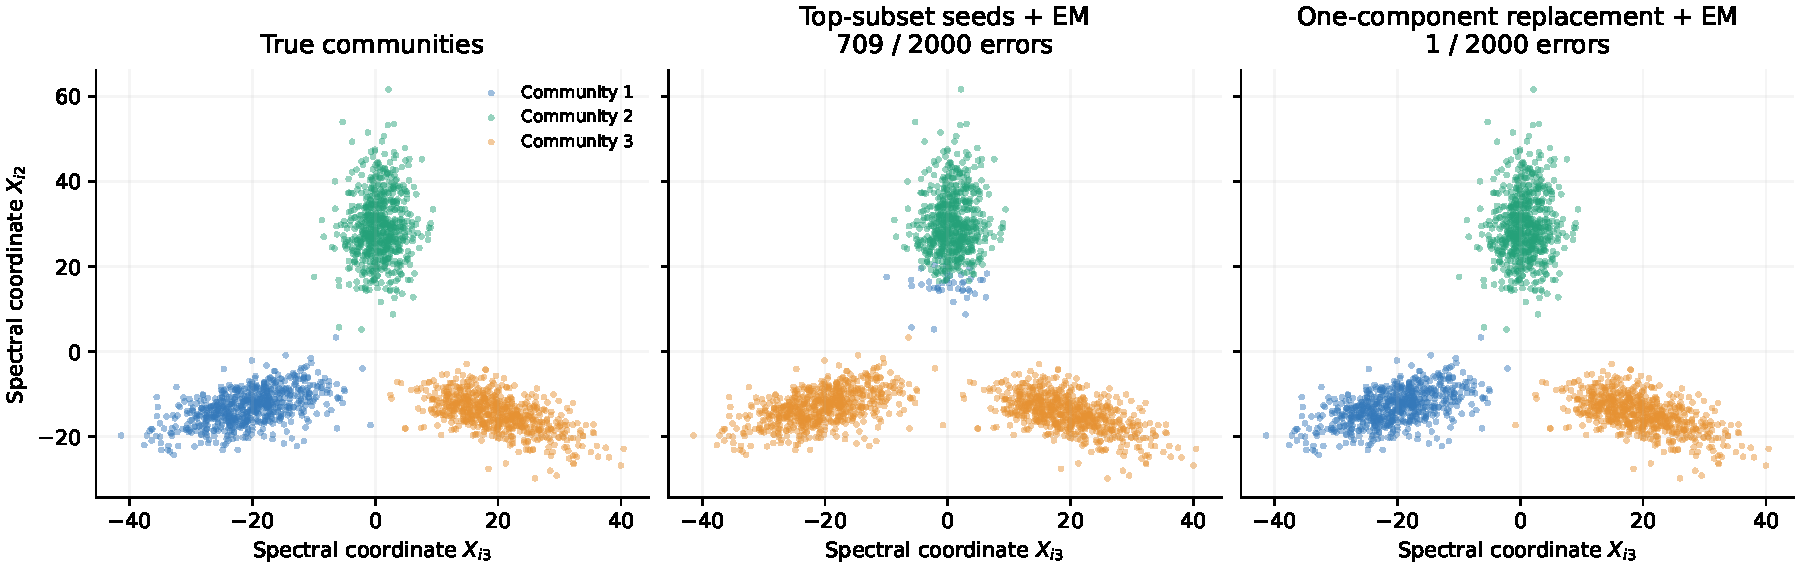
\includegraphics[width=\linewidth]{figures/initialization_failure_repair.pdf}
\caption{The saved design failure, displayed in two coordinates of
$X=\sqrt n U\Lambda$. Left: true communities, used only for evaluation.
Middle: top-subset peeling followed by EM merges the two lower communities
and splits the upper community. Right: an accepted one-component replacement
followed by EM separates the groups and leaves one mislabeled node. Predicted
labels are aligned to truth for display only.}
\label{fig:initialization_repair}
\end{figure}

\subsection{Historical numerical verification and computational scope}

All returned historical profile fits satisfy the declared stopping rule in the 240-graph
comparison. The 120 original peeling errors are reproduced exactly. The
archive contains 6240 EM traces, including replacement proposals, growing
stages, and restart fits, with 27867 recorded trace points. The smallest
observed objective increment is $-1.17\times10^{-10}$, within floating-point
rounding; no increment below $-10^{-7}$ occurs. All 240 selected ten-start
solutions maximize the same final working likelihood within their restart
set. Replacement accepts a likelihood improvement on 22 design graphs and
25 independent graphs, and never lowers the final objective; most of these
small improvements do not change the classification error. Independent
scalar checks reproduce deviance and global-gain calculations with maximum
absolute errors $7.11\times10^{-15}$ and $1.78\times10^{-15}$, respectively.

The present implementation explicitly reconstructs the $n\times n$ profiles
and caches all singleton-candidate scores. Reconstruction costs
$O(n^2K)$, score precomputation costs $O(n^3)$, and storage costs $O(n^2)$.
An EM update costs $O(n^2K)$. A replacement pass tries $K$ additional fits,
whereas ten-start residual seeding uses ten fits. The runs use one numerical
library thread per worker and four worker processes. Python, NumPy, SciPy,
and scikit-learn versions are 3.11.7, 2.1.3, 1.16.2, and 1.7.1. Stored timers
cover all candidate arms and restarts together and exclude graph generation
and eigenpair computation, so they do not support an arm-specific speed
claim. The data sizes $n\le2000$ establish feasibility for this implementation;
candidate-pool approximations and blockwise computations require separate
large-graph validation.

The archived comparisons support improved decoding of a fixed spectrum in
several heterogeneous models and identify a concrete failure of subset
initialization. The new 60-graph study directly evaluates the current
Algorithm~1 and records its weak-signal failures and its lack of a substantive
replacement improvement on that particular collection. Neither collection
estimates an asymptotic error exponent, proves uniform dominance over
$k$-means, or replaces the model assumptions and analysis of
Theorems~\ref{thm:main-recovery} and~\ref{thm:local-spectral-em}.

\paragraph{Companion sparse threshold-certificate checks.}
A separately retained sparse-score implementation tests a uniform-weight
refit together with the replacement trials and accepts only gains of at
least $(\sum_{ij}q_{ij})/\sqrt{\log n}$. Its archived checks contain 24
graphs with $n\in\{256,512\}$, $K\in\{3,4,6\}$, two degree scales,
and two seeds in one heterogeneous assortative family. They record 19 exact
recoveries and seven errors among 9,216 nodes; no natural growing endpoint
requires an accepted replacement in that collection. A separate injected
collapsed population endpoint is repaired in two accepted rounds. These
checks concern the companion sparse threshold rule, not the complete
Bernoulli Algorithm~1. They remain available as
\path{general_k_fresh_checks.json} beside that implementation.
